\section{Study Design and Data Collection}
\label{sec:study-design}
To understand the decision making factors and reasoning patterns of a diverse population regarding AI use cases, we conducted a survey-based study with demographically diverse participants. In this section, we discuss the selection of use cases (\S~\ref{ssec:use-cases}), survey design (\S~\ref{ssec:survey-design}), and data collection details and participant demographics (\S~\ref{ssec:data-and-demographics}).

\subsection{Use Cases}
\label{ssec:use-cases}
% We define an AI use case as one where an AI system replaces a specific role or function, and we follow three of the five concepts used in EU AI Act to describe each use case \citep{golpayegani2023risk}: the domain, purpose, and capabilities. 
% \jana{Should be consistent in the following sections about whether we call the use case categories "AI in professional usage" or "AI in labor replacement" (I personally prefer the latter).  Also might want to consider calling the "personal" category "personal healthcare".  Also, in Fig. 1, it's not clear what "Pre-survey Question" and "Post-survey Question" mean.} 
To understand how different characteristics of AI use cases can impact judgments and decision making processes, we crafted ten different AI use cases. We first chose two broad application categories frequently mentioned by the public in previous works \citep{kieslich2024myfuture,mun2024participaidemocraticsurveyingframework}: \textbf{AI in personal}, everyday usage where participants could uniformly consider themselves as AI users and \textbf{AI in professional usage} where AI takes on a role thus far done by a human as a profession, e.g., Lawyer AI. We then developed five use cases in the AI in professional usage category that varied according to the level of education required for entry and five use cases in AI in personal category that varied according to the risk level assigned by the EU AI act. All the personal use cases were in the health domain, reflecting a key domain of interest conveyed by lay users in previous works \citep{mun2024participaidemocraticsurveyingframework,kieslich2024myfuture}.
% In the use case descriptions, we focus on text-based, non-embodied, digital systems, to ensure that an AI system can fully replace the role/function online.

\subsection{Use Cases Specialization}\label{sec:usecase}

\begin{figure}
    \centering    
{\footnotesize
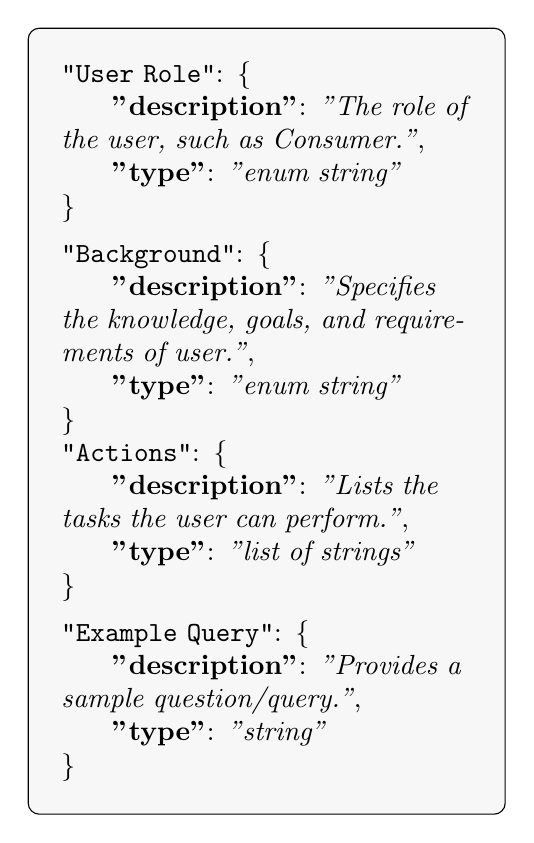
\begin{tikzpicture}
% Draw rounded rectangle with shadow
\node[rectangle, rounded corners, draw=black, fill=black!3!white, text width=0.43\textwidth, inner sep=12pt, align=left] (box) {
    \textbf{\texttt{"User Role"}}: \{\\
    \hspace{15pt} \textbf{"description"}: \textit{"The role of the user, such as Consumer."}, \\
    \hspace{15pt} \textbf{"type"}: \textit{"enum string"} \\
    \} \vspace{5pt}\\
    \textbf{\texttt{"Background"}}: \{\\
    \hspace{15pt} \textbf{"description"}: \textit{"Specifies the knowledge, goals, and requirements of user."}, \\
    \hspace{15pt} \textbf{"type"}: \textit{"enum string"} \\
    \} \\
    \textbf{\texttt{"Actions"}}: \{\\
    \hspace{15pt} \textbf{"description"}: \textit{"Lists the tasks the user can perform."}, \\
    \hspace{15pt} \textbf{"type"}: \textit{"list of strings"} \\
    \} \vspace{5pt}\\
    \textbf{\texttt{"Example Query"}}: \{\\
    \hspace{15pt} \textbf{"description"}: \textit{"Provides a sample question/query."}, \\
    \hspace{15pt} \textbf{"type"}: \textit{"string"} \\
    \}
};

\end{tikzpicture}
}
\caption{Use case specializations. For each use case, we define its role, goal, actions, and example query. For each property, we present its description and type.}
\label{fig:usecasedef}
\end{figure}

\begin{table*}[]
\centering
\caption{The actions and example query for each kind of user role defined for \chatiot.}
\label{tab:usecase}
\resizebox{\textwidth}{!}{

\begin{tabular}{p{1.5cm}|p{12cm}|p{4cm}}
%\begin{tabular}{@{}c@{\hskip 0.1cm}|
%    @{\hskip 0.1cm}>{\arraybackslash}p{10.5cm}@{\hskip 0.1cm}|
%    @{\hskip 0.1cm}>{\arraybackslash}p{5cm}@{\hskip 0.1cm}
%    }
\toprule
\toprule
\multicolumn{1}{c|}{Role} & \multicolumn{1}{c|}{Actions} & \multicolumn{1}{c}{Example Query}  \\ \midrule
Consumer  
& \romannumeral1) Assess the security of IoT devices before purchase or installation; \newline
\romannumeral2) Monitor ongoing security status and updates for existing devices;\newline
\romannumeral3) Make informed decisions based on security reports provided by \chatiot.
& Is it secure to use Signify Smart Lighting in home? \\
\midrule

Security Analyst  
&
\romannumeral1) Identify and evaluate security threats and vulnerabilities in IoT devices;\newline
\romannumeral2) Recommend mitigation strategies based on threat intelligence and analysis;\newline
\romannumeral3) Provide detailed security reports to stakeholders.
& Conduct a security assessment for TP-Link AX6000 Wi-Fi 6 Router. 
\\ \midrule

Technical Officer 
&
\romannumeral1) Ensure that IoT devices are deployed securely and operate within compliance guidelines;\newline
\romannumeral2) Oversee the application of security updates and patches;\newline
\romannumeral3) Monitor the security posture of the IoT ecosystem within their organization.
& Check the security labeling of the company's WiFi Routers,  including TP-Link, D-Link, and ASUS in Singapore. 
\\
\midrule

Developer
&
\romannumeral1) Design and develop secure IoT products by adhering to best practices and security standards;\newline
\romannumeral2) Continuously update products to address new vulnerabilities and threats;\newline
\romannumeral3) Provide accurate security documentation and updates to customers.
&
Develop a security enhancement roadmap for the next generation of TP-Link Wi-Fi routers.
\\
\midrule

Trainer 
&
\romannumeral1) Develop and deliver training programs on IoT security;\newline
\romannumeral2) Guide users and organizations on how to secure IoT devices and respond to incidents;\newline
\romannumeral3) Provide up-to-date information on IoT security trends and best practices.
&
Prepare a guide on the importance of cybersecurity labeling for smart locks like the August Smart Lock.
\\
\bottomrule
\bottomrule

\end{tabular}}
\end{table*}

In this section, we define five specialized use cases of \chatiot. 
Each use case is defined by \textit{four} fundamental properties: \textit{User Role}, \textit{Background}, \textit{Actions}, and \textit{Example Query}, within the IoT security domain.
The detailed specifications are illustrated in Figure~\ref{fig:usecasedef}.
The roles include \textit{Consumer}, \textit{Security Analyst}, \textit{Technical Officer}, \textit{Developer}, and \textit{Trainer}. 
Recall that we have discussed background in \S~\ref{sec:resgen}, we present the detailed actions and example query in the following context.


Table~\ref{tab:usecase} highlights the key actions associated with each user role, such as assessing the security of IoT devices, deploying security patches, or developing training programs on IoT security.
Additionally, it provides example queries for each role, demonstrating how \chatiot\ can be utilized to address the unique needs of various users. 
This structured approach ensures that \chatiot\ caters to a diverse range of users, offering tailored assistance and enhancing IoT security management across different scenarios.
Note that while we provide five use cases, they are not rigid or fixed. 
The use cases can be easily extended by defining new user roles, specifying the background (including knowledge, goals, and requirements), and outlining actions. Example queries can also be added to further clarify the context and functionality of each user role.


\paragraph{Professional Use Case Scenarios} 
For the first area of focus, AI in labor replacement, we collected jobs listed in the U.S. census bureau\footnote{https://www.bls.gov/ooh/occupation-finder.htm} and sorted them according to entry level education required as stated in the census. We chose education level as it has been tightly linked to socioeconomic and occupational status \citep{svensson2006professional,evetts2006introduction}. We selected jobs that have a large portion of digital or intellectual components with minimal requirement for embodiment resulting in following five professional roles: Lawyer, Elementary school teacher, IT support specialist, Government support eligibility interviewer, and Telemarketer. See Table~\ref{tab:use-cases} for further details.

\paragraph{Personal Use Case Scenarios} 
 To understand the acceptability of different health applications in personal and private life, we adapted the descriptions of personal use cases written by participants from prior works \citep{mun2024participaidemocraticsurveyingframework,kieslich2024myfuture}. The research team iteratively refined the descriptions to reflect risk levels according to EU AI Act, and  confirmed agreement with categories assigned by GPT-4, following \citeauthor{herdel2024exploregen}. See Table~\ref{tab:use-cases} for further details.

\subsection{Survey Design}
\label{ssec:survey-design}
Our survey presents participants with five use case descriptions, all from either the professional or personal category (randomly assigned and presented in random order) (see \S~\ref{ssec:use-cases} for details). After each description, participants answer: "Do you think a technology like this should be developed?" (Q1) and then, "How confident are you in your above answer?" (Q2). They provide open-text rationales by completing the prompt, "[Use Case] should be developed because..." (Q3), tailored to their Q1 response ("should" for "Yes" and "should not" for "No"). Participants also specify a condition for switching their decision with, "[Use Case] should not be developed if..." (Q4), adjusted similarly to Q1. Subsequently, they answer, "If [Use Case] existed, would you use its service?" (Q5) and express confidence with, "How confident are you in your above answer?" (Q6). Refer to Table~\ref{app:part-1-questions} in the Appendix for the exact wording of the questions.
% \jana{The next part should be written in a way that is consistent with the Intro.  For ex, if we are still using the Study 1/Study 2 language, call the second one Study 2.  Also repeat the same rationale given in the Intro for the 2nd study.} In addition to the main survey, we crafted and conducted a variation asking participants to explicitly list and weigh harms and benefits of a use case to understand whether such process impacts judgment. We further detail survey questions and design for both surveys in Appendix~\ref{app:survey-details}.

\paragraph{Collecting Participant Characteristics}
Following the main survey, we asked participants questions about their AI literacy and demographics to explore various factors affecting perception of AI acceptance. We adopted a shortened version of AI literacy questionnaires from previous works \citep{wang2023measuring,mun2024participaidemocraticsurveyingframework} with four AI literacy aspects, AI awareness, usage, evaluation, and ethics, and two additional questions for generative AI, usage frequency and familiarity with limitations. We collected demographic information of the participants such as race, gender, age, sexual orientation, religion, employment status, income, and level of education. Additionally, we collected information about chronicity, i.e., prolonged experiences of everyday discrimination, of their discrimination experiences (if any) following \citeauthor{kingsley2024investigating}.  
% \jana{add a brief phrase explaining what chronicity means.} 
% To further understand the decision making styles of participants that could inform AI acceptability judgments, we included three questionnaires in our survey: Moral foundations questionnaire \citep{graham2008moral}, Oxford Utilitarianism Scale \citep{kahane2018beyond}, and Toronto empathy questionnaire \citep{spreng2009toronto}.

\subsection{Data Collection and Participant Demographics}
\label{ssec:data-and-demographics}
We used Prolific\footnote{https://www.prolific.com} to recruit participants. To represent diverse sample, we stratified our recruitment by the ethnicity categories (White, Mixed, Asian, Black and Other) and age (18-48, 49-100) provided by Prolific. We also added criteria for quality such as survey approval rating and number of previous surveys completed.
% \jana{usually best practice to say exactly what criteria you used, rather than "etc."} 
Our study was approved by IRB at our institutions, and we paid 12 USD/hour. Our final sample consisted of 197 participants across two categories, with professional usage assigned to 100 participants and personal to 97. See Appendix~\ref{app:participant-details} for further details on participants.

\section{Analysis Methods}
Our surveys consisted of both multiple choice (numerical) and open-text questions designed to answer our research questions. In this section, we detail our process for numerical (\S~\ref{ssec:num-analysis}) and open-text (\S~\ref{ssec:text-analysis}) analysis.

\subsection{Multiple Choice Analysis}
\label{ssec:num-analysis}
% \maarten{Might be good to discuss these in terms of the question numbers they come from (like you did below)? Also, I think an example or two would be nice? Or a formula? cause "converted to numerical value, multiplied, and scaled" sounds a little confusing?}
% \jana{Maybe multiple choice analysis instead of numerical analysis?  And then phrase the text as "We analyzed the judgment and confidence ratings by..."?} 
We analyzed the judgment and confidence ratings by mapping judgment (Q1, Q5) to 1 (``Should be developed'', ``Would use'') or -1 (``Should not be developed'', ``Would not use'') and confidence (Q2, Q6) to a scale from 1 to 5. We used numerically converted judgment, confidence, and combined (judgment$\times$confidence; -5 to 5) values as dependent variables in our analysis. We used repeated-measures ANOVAs to understand the differences in mean responses between conditions/groups and linear mixed effects regression models (lmer) to better understand the effects of specific factors. We included a subject-specific random effect when using ANOVA and regression models and added a use-case-specific random effect when applicable. We factorized demographic responses for analysis with the exception of discrimination chronicity, which we aggregated to a numerical value \citep{kingsley2024investigating, michaels2019coding}. We also converted responses to AI literacy questions to numerical values for analysis. 
% do a little more reading on how we should present what we did
\subsection{Open-response Analysis}
\label{ssec:text-analysis}
To assess the reasoning methods used by the participants, we analyzed the open-text responses on elaborations to their decisions (Q3) and circumstances in which their decisions would switch (Q4) along the following three dimensions: reasoning types (cost-benefit, rule-based, both, unclear), reference to moral foundations (Care, Fairness, Purity, Authority, Loyalty), and switching conditions (Functionality, Usage, Societal Impact). By analyzing reasoning types and moral values reflected in the participants' justifications, we aim to characterize \emph{how} participants made their decisions, and by analyzing various factors such as primary concerns and stakeholders, we aim to discover \emph{what} aspects were salient for the participants in their decisions. \looseness=-1

% \wesley{Given the page limit, we might want to give an one paragraph summarization of the following subsections, and leave most of the texts in Appendix under "Additional Analysis Details" Wondering what's your thought on this, Jimin and Maarten!}

% \paragraph{Annotation Dimensions}
% \label{sssec:annotation-dim}
%  \jana{It would read to me better if the rationale and citations for why we chose these categories go in the intro, and this section be reserved for information about how the classifications were achieved.} Inspired by previous works in moral psychology, we used two main reasoning types to characterize participants' decision making pattern as expressed in their open-text answers: cost-benefit reasoning and rule-based reasoning \citep{cheung2024measuring}. Furthermore, we used five moral values \citep[care, fairness, loyalty, authority, and purity;][]{graham2011mapping,graham2008moral} to annotate underlying values in participants' reasoning\footnote{While these dimensions have been re-defined to include more diverse values from participants beyond WEIRD (white, educated, industrialized, rich, and democratic) \citep{atari2023morality}, we used these five dimensions to mirror our survey design.}. Moreover, we annotated concerns expressed in switching conditions using three categories \jana{note that many reviewers will want more clarity about what the intended definition of these categories are...can we provide a short phrase that summarizes the definition of each one before giving the examples?}: functionality (e.g., errors, bias in systems, limited capabilities), usage (e.g., misuse and unintended use), and societal impact (e.g., job loss, over-reliance), inspired by harm taxonomy developed by \citeauthor{solaiman2023evaluating} and user concern annotation practice adopted by \citeauthor{mun2024participaidemocraticsurveyingframework}.

\paragraph{Classification and Aggregation} 
We classified participants' responses to Q3 (elaboration of judgment) and Q4 (conditions for switching decisions) using OpenAI's o1-mini\footnote{\texttt{o1-mini-2024-09-12}}. To validate the model's classification performance, results were compared with a reference set of 100 samples annotated by three independent annotators, comprised of team members and a professional annotator. Initially, each annotator independently assessed the data, and then consensus was reached through discussion to establish a gold standard set. The inter-rater agreement between the gold standard and o1-mini's annotations was evaluated using Gwet's AC1 metric, chosen for its robustness with infrequent labels \citep{wongpakaran2013comparison}. The agreement levels varied, ranging from moderate to almost perfect with no dimension below moderate. Annotations for cost-benefit reasoning, rule-based reasoning, and authority reached near-perfect agreement; purity and usage achieved substantial agreement; the rest showed moderate agreement.
% \jana{should also state briefly which ones only had moderate agreement}. 
Due to a lack of sufficient test samples and minimal occurrences in the annotated data, the moral value dimension Loyalty was excluded from further analysis. The annotations were converted into a one-hot encoding format for statistical analysis. See Appendix~\ref{app:open-text-annotation-details} for further details.
% See App~\ref{tab:irr-results} for further details. We presented answers to both questions together as coherent text along with the use case description; see Appendix~\ref{app:placeholder} for details on prompts and settings.